\section{Rutas y órdenes de trabajo}


Despacho de lecturas, instalaciones y operación de campo.


\begin{quote}
\textbf{Ficha de dominio:} documenta períodos, rutas, órdenes de trabajo y operaciones del personal de campo, incluida la vinculación de lecturas y la evidencia externa.
\end{quote}


\subsection{Alcance y entradas HTTP}


\begin{itemize}
\item \textbf{Controladores:} \texttt{\detokenize{RoutesController}}, \texttt{\detokenize{OrdenesTrabajoController}}, \texttt{\detokenize{OperatorController}}.
\item \textbf{Servicios:} \texttt{\detokenize{RoutesService}}, \texttt{\detokenize{OrdenesTrabajoService}}.
\item \textbf{Casos:} \texttt{\detokenize{CreateRouteUseCase}}, \texttt{\detokenize{FindAllRoutesUseCase}}, \texttt{\detokenize{FindOneRouteUseCase}}, \texttt{\detokenize{UpdateRouteUseCase}}, \texttt{\detokenize{DeleteRouteUseCase}}, \texttt{\detokenize{ReassignRouteUseCase}}, \texttt{\detokenize{GetEligibleReadingsUseCase}}, \texttt{\detokenize{GetReadingsByRutaUseCase}}, \texttt{\detokenize{FindOrdenesByRutaUseCase}}, \texttt{\detokenize{ExportFieldSheetPdfUseCase}}, \texttt{\detokenize{UpdateOrdenEstadoUseCase}}, \texttt{\detokenize{LinkLecturaUseCase}}, \texttt{\detokenize{GetOperatorRoutesUseCase}}, \texttt{\detokenize{UpdateRouteStateUseCase}}, \texttt{\detokenize{UpdateOperatorWorkOrderUseCase}}.
\item Los períodos se consultan directamente desde \texttt{\detokenize{RoutesService}}; no se confirmó caso dedicado para listar rutas administrativas ni para algunos cambios de órdenes.
\end{itemize}

\subsection{Comportamiento de negocio verificable}
Las tablas relacionadas son \texttt{Rutas}, \texttt{OrdenTrabajo}, \texttt{EjecucionOrdenTrabajo}, \texttt{Lecturas}, \texttt{Periodos} y \texttt{NovedadOrdenTrabajo}. El flujo confirmado es período $\rightarrow$ ruta $\rightarrow$ orden $\rightarrow$ lectura/evidencia $\rightarrow$ cierre. No se encontró fórmula monetaria que aplique a este módulo. La promoción automática del contrato a \texttt{ACTIVO} al completar orden de instalación \textbf{sí} está implementada --- ver \texttt{02-contratos.md}, sección ``Transiciones de estado del contrato''.


\begin{center}
\small
\begin{longtable}{|p{0.313\textwidth}|p{0.313\textwidth}|p{0.313\textwidth}|}
\hline
\textbf{Método y ruta} & \textbf{Caso/servicio ejecutado} & \textbf{Resultado} \\
\hline
\endfirsthead
\hline
\textbf{Método y ruta} & \textbf{Caso/servicio ejecutado} & \textbf{Resultado} \\
\hline
\endhead
\texttt{\detokenize{GET /api/v1/routes/periods}} & \texttt{\detokenize{RoutesService.getPeriodos()}} & Períodos. \\
\hline
\texttt{\detokenize{GET /api/v1/routes/eligible-readings}} & \texttt{\detokenize{getEligibleReadings()}} → \texttt{\detokenize{GetEligibleReadingsUseCase}} & Lecturas elegibles paginadas. \\
\hline
\texttt{\detokenize{GET /api/v1/routes/:rutaId/readings}} & \texttt{\detokenize{getReadingsByRuta()}} → \texttt{\detokenize{GetReadingsByRutaUseCase}} & Lecturas de ruta. \\
\hline
\texttt{\detokenize{POST /api/v1/routes}} & \texttt{\detokenize{create()}} → \texttt{\detokenize{CreateRouteUseCase}} & Ruta creada. \\
\hline
\texttt{\detokenize{GET /api/v1/routes}} / \texttt{\detokenize{:id}} & \texttt{\detokenize{findAll()}} / \texttt{\detokenize{findOne()}} → casos de consulta & Rutas. \\
\hline
\texttt{\detokenize{PATCH /api/v1/routes/:id}} & \texttt{\detokenize{update()}} → \texttt{\detokenize{UpdateRouteUseCase}} & Ruta actualizada. \\
\hline
\texttt{\detokenize{PATCH /api/v1/routes/:id/reassign}} & \texttt{\detokenize{ReassignRouteUseCase.execute()}} & Operario reasignado. \\
\hline
\texttt{\detokenize{DELETE /api/v1/routes/:id}} & \texttt{\detokenize{delete()}} → \texttt{\detokenize{DeleteRouteUseCase}} & Soft delete. \\
\hline
\texttt{\detokenize{GET /api/v1/routes/:id/pdf}} & \texttt{\detokenize{ExportFieldSheetPdfUseCase}} & PDF. \\
\hline
\texttt{\detokenize{GET /api/v1/routes/:id/work-orders}} & \texttt{\detokenize{FindOrdenesByRutaUseCase}} & Órdenes paginadas. \\
\hline
\texttt{\detokenize{PATCH /api/v1/work-orders/:id/state}} & \texttt{\detokenize{UpdateOrdenEstadoUseCase}} & Estado de orden. \\
\hline
\texttt{\detokenize{PATCH /api/v1/work-orders/:id/reading}} & \texttt{\detokenize{LinkLecturaUseCase}} & Lectura vinculada. \\
\hline
\texttt{\detokenize{GET/PATCH /api/v1/operator/routes...}} & \texttt{\detokenize{GetOperatorRoutesUseCase}} / \texttt{\detokenize{UpdateRouteStateUseCase}} & Vista y estado del operador. \\
\hline
\texttt{\detokenize{PATCH /api/v1/operator/work-orders/:id}} & \texttt{\detokenize{UpdateOperatorWorkOrderUseCase}} & Ejecución/evidencia. \\
\hline
\end{longtable}
\end{center}


\subsection{Ejemplo JSON}


\begin{lstlisting}
{
  "rutaId": "42",
  "nombre": "Lecturas agosto",
  "tipoRuta": "LECTURA",
  "estado": "PENDIENTE",
  "ordenesTrabajo": []
}
\end{lstlisting}


\begin{center}
\small
\begin{longtable}{|p{0.313\textwidth}|p{0.313\textwidth}|p{0.313\textwidth}|}
\hline
\textbf{Campo} & \textbf{Tipo} & \textbf{Regla/uso} \\
\hline
\endfirsthead
\hline
\textbf{Campo} & \textbf{Tipo} & \textbf{Regla/uso} \\
\hline
\endhead
\texttt{\detokenize{rutaId}}, \texttt{\detokenize{ordenTrabajoId}}, \texttt{\detokenize{lecturaId}} & string & \texttt{\detokenize{BigInt}} serializado. \\
\hline
\texttt{\detokenize{tipoRuta}} & enum & Actividad de la ruta. \\
\hline
\texttt{\detokenize{estado}} & enum & Estado de ruta u orden según el DTO. \\
\hline
\texttt{\detokenize{operarioId}}, \texttt{\detokenize{periodoId}}, \texttt{\detokenize{comunidadId}} & number/null & Asignación y contexto. \\
\hline
\texttt{\detokenize{ordenesTrabajo}} & array & Órdenes asociadas. \\
\hline
\end{longtable}
\end{center}


\subsection{Estados}


\begin{center}
\small
\begin{longtable}{|p{0.313\textwidth}|p{0.313\textwidth}|p{0.313\textwidth}|}
\hline
\textbf{Entidad} & \textbf{Estados confirmados} & \textbf{Significado} \\
\hline
\endfirsthead
\hline
\textbf{Entidad} & \textbf{Estados confirmados} & \textbf{Significado} \\
\hline
\endhead
Ruta & \texttt{\detokenize{PENDIENTE}}, \texttt{\detokenize{EN_PROGRESO}}, \texttt{\detokenize{COMPLETADA}}, \texttt{\detokenize{PARCIAL}}, \texttt{\detokenize{CANCELADA}} & Pendiente, ejecutada, finalizada, incompleta o cancelada. \\
\hline
Orden & \texttt{\detokenize{PENDIENTE}}, \texttt{\detokenize{EN_PROGRESO}}, \texttt{\detokenize{COMPLETADA}}, \texttt{\detokenize{CANCELADA}}, \texttt{\detokenize{FALLIDA}} & Ciclo de trabajo. \\
\hline
\end{longtable}
\end{center}

\subsubsection{Máquina de estados de la Ruta}

La máquina está implementada como una tabla de transiciones explícita en \texttt{backend/src/operations/routes/domain/route-state.ts}:

\begin{center}
\small
\begin{longtable}{|p{0.30\textwidth}|p{0.65\textwidth}|}
\hline
\textbf{Desde} & \textbf{Hacia permitidas} \\
\hline
\endfirsthead
\hline
\textbf{Desde} & \textbf{Hacia permitidas} \\
\hline
\endhead
\texttt{\detokenize{PENDIENTE}} & \texttt{\detokenize{EN_PROGRESO}}, \texttt{\detokenize{CANCELADA}} \\
\hline
\texttt{\detokenize{EN_PROGRESO}} & \texttt{\detokenize{COMPLETADA}}, \texttt{\detokenize{PARCIAL}}, \texttt{\detokenize{PENDIENTE}}, \texttt{\detokenize{CANCELADA}} \\
\hline
\texttt{\detokenize{COMPLETADA}} & \texttt{\detokenize{EN_PROGRESO}} (reabre para corrección de cierre) \\
\hline
\texttt{\detokenize{PARCIAL}} & \texttt{\detokenize{EN_PROGRESO}} (reabre para continuar trabajo) \\
\hline
\texttt{\detokenize{CANCELADA}} & \texttt{\detokenize{PENDIENTE}} (reabre para reactivación) \\
\hline
\end{longtable}
\end{center}

La función \texttt{canTransitionRouteState(from, to)} valida la transición; \texttt{UpdateRouteUseCase.execute()} rechaza con \texttt{InvalidDomainOperationException} si la transición no está permitida. \textbf{No existe máquina equivalente para OrdenTrabajo} --- sus transiciones las acepta todas \texttt{UpdateOrdenEstadoUseCase} mientras el estado pertenezca al enum.


\subsection{Regla de novedades sin estado adicional de orden}

\textbf{Decisión funcional propuesta — pendiente de implementación.} No se agregará un estado persistido \texttt{NOVEDAD} a \texttt{OrdenTrabajo}. Mientras exista una novedad, la orden permanece en \texttt{EN\_PROGRESO}; la interfaz muestra una alerta derivada al consultar la relación de novedades activas.

\subsubsection{Flujo acordado de orden con novedad}

\begin{figure}[h]
\centering
\IfFileExists{images/04-orden-lectura-flujo.png}{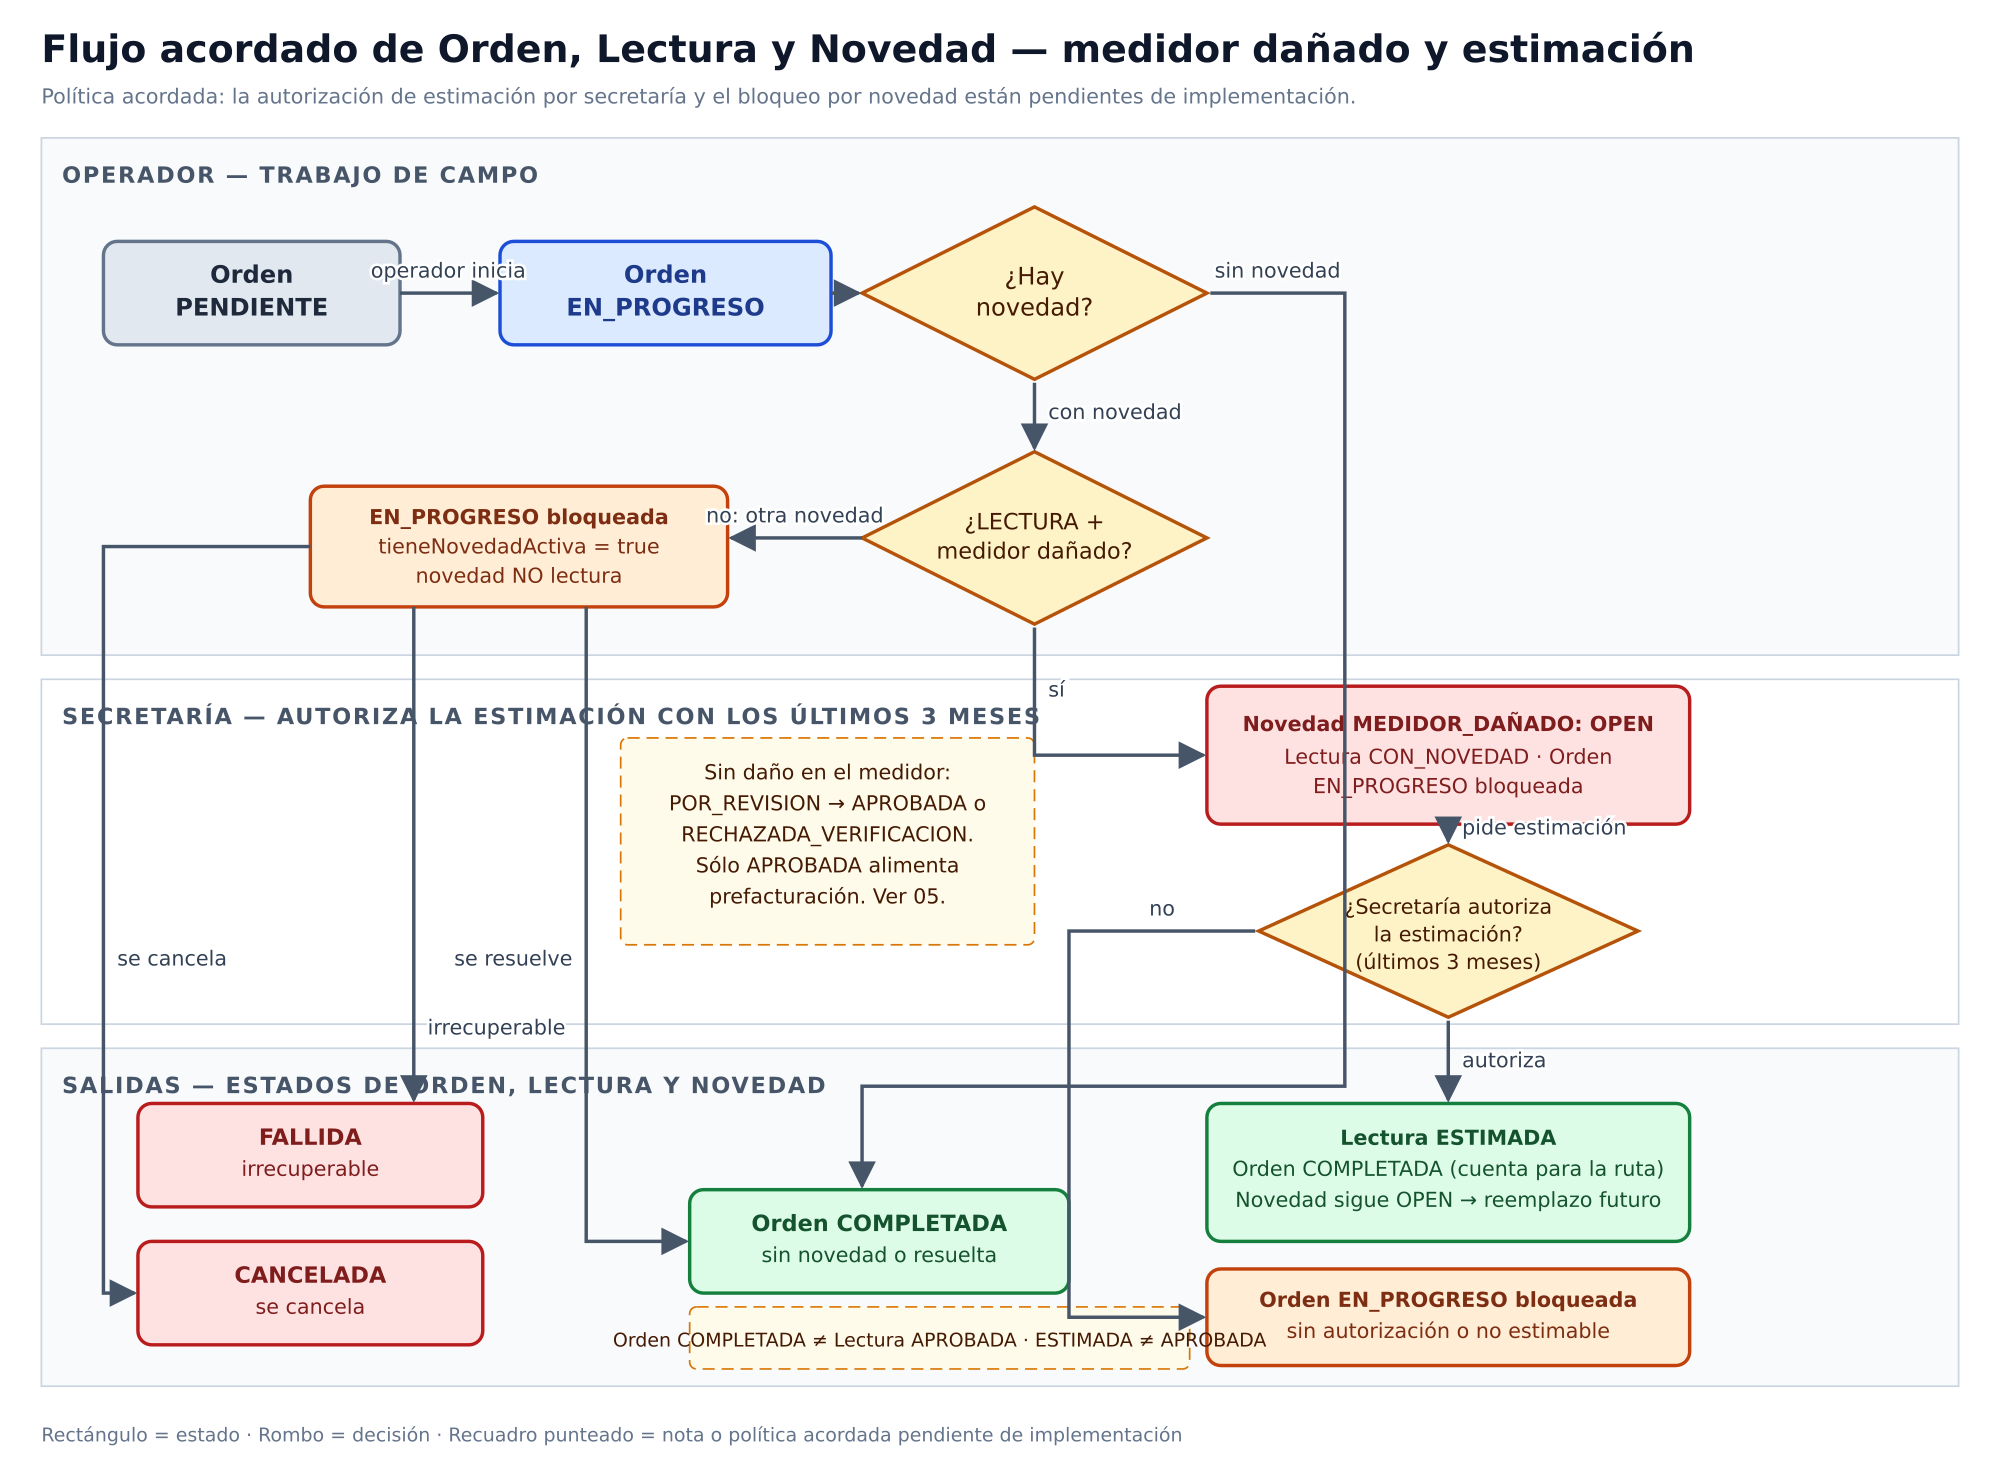
\includegraphics[width=0.95\textwidth]{images/04-orden-lectura-flujo.png}}{\fbox{\parbox{0.88\textwidth}{\centering Flujo acordado: PENDIENTE $\rightarrow$ EN\_PROGRESO $\rightarrow$ COMPLETADA; bloqueo por novedad con {\ttfamily tieneNovedadActiva}; salidas FALLIDA/CANCELADA; estimación autorizada por secretaría.\\[3pt]Agregar \texttt{images/04-orden-lectura-flujo.png} para reemplazar este fallback.}}}
\caption{Flujo acordado de orden, lectura y novedad. Fuente editable: {\ttfamily diagrams/orden-lectura-novedad.drawio}.}
\end{figure}

Resumen textual del flujo:
\begin{itemize}
\item La orden inicia en \texttt{PENDIENTE}; el operador la pasa a \texttt{EN\_PROGRESO} al iniciar el trabajo.
\item Sin novedad, la orden se completa (\texttt{COMPLETADA}).
\item Con novedad en una orden que NO es de lectura, la orden queda en \texttt{EN\_PROGRESO} con \texttt{tieneNovedadActiva=true} hasta resolverla; si el caso es irrecuperable pasa a \texttt{FALLIDA}, y si se cancela pasa a \texttt{CANCELADA}.
\item En una orden de \texttt{LECTURA} con medidor dañado, el operador crea una \texttt{NovedadOrdenTrabajo} en \texttt{OPEN}; la lectura queda en \texttt{CON\_NOVEDAD} y la orden permanece en \texttt{EN\_PROGRESO} bloqueada.
\item Sólo secretaría puede autorizar la estimación con los últimos 3 meses (\textbf{política acordada, pendiente de implementación}): si autoriza, la lectura pasa a \texttt{ESTIMADA} y la orden a \texttt{COMPLETADA}, mientras la novedad sigue en \texttt{OPEN} para un reemplazo futuro; si no autoriza o no se puede estimar, la orden sigue bloqueada.
\item La orden \texttt{COMPLETADA} no implica lectura \texttt{APROBADA}: la estimación genera \texttt{ESTIMADA}, no \texttt{APROBADA}.
\item La orden completada por estimación autorizada cuenta como \texttt{COMPLETADA} para el cierre de la ruta.
\end{itemize}

\texttt{NOVEDAD} no es un valor del enum de \texttt{OrdenTrabajo}: es una condición derivada de la relación con \texttt{NovedadOrdenTrabajo} y de la existencia de novedades activas. No debe persistirse ni confundirse con \texttt{OrdenTrabajo.estado}.

\subsubsection{Tres máquinas separadas}

\begin{center}
\small
\begin{longtable}{|p{0.25\textwidth}|p{0.34\textwidth}|p{0.31\textwidth}|}
\hline
\textbf{Entidad} & \textbf{Máquina} & \textbf{Responsabilidad} \\
\hline
\endfirsthead
\hline
\textbf{Entidad} & \textbf{Máquina} & \textbf{Responsabilidad} \\
\hline
\endhead
\texttt{OrdenTrabajo.estado} & Ejecución operativa: \texttt{PENDIENTE}, \texttt{EN\_PROGRESO}, \texttt{COMPLETADA}, \texttt{CANCELADA}, \texttt{FALLIDA}. & Etapa del trabajo de campo y cierre de la orden. \\
\hline
\texttt{NovedadOrdenTrabajo.estado} & Análisis de anomalía: \texttt{OPEN}, \texttt{IN\_PROGRESS}, \texttt{RESOLVED}, \texttt{CANCELLED}. & Atención, resolución o cancelación de la anomalía. \\
\hline
\texttt{Lectura.estado} & Captura y validación: \texttt{PENDIENTE}, \texttt{POR\_REVISION}, \texttt{APROBADA}, \texttt{RECHAZADA\_VERIFICACION}, \texttt{ESTIMADA}, \texttt{PLANILLADA}, \texttt{CON\_NOVEDAD}. & Ciclo de captura, revisión, aprobación, rechazo o tratamiento del dato. \\
\hline
\end{longtable}
\end{center}

Una novedad activa puede generar una alerta sobre la orden, pero no transforma su estado persistido en \texttt{NOVEDAD}; una lectura con \texttt{CON\_NOVEDAD} tampoco reemplaza el estado de la orden ni el estado de la novedad.

\subsubsection{Ejemplo de respuesta derivada}

\begin{lstlisting}
{
  "ordenTrabajoId": "9",
  "estado": "EN_PROGRESO",
  "tieneNovedadActiva": true,
  "novedadesActivas": [
    {
      "novedadOrdenTrabajoId": "31",
      "estado": "OPEN",
      "tipo": "LECTURA_ERRONEA",
      "observacion": "El visor no permite validar el consumo"
    }
  ]
}
\end{lstlisting}

\subsubsection{Regla de backend y pendiente funcional}

La UI no es la única barrera. Como regla de backend propuesta, una operación no debe permitir pasar la orden a \texttt{COMPLETADA} si existe una novedad abierta que afecte el resultado; la validación debe ejecutarse en el caso de uso o repositorio que completa la orden. Esta regla está pendiente de implementación.

También está pendiente definir el campo o criterio que determina si una novedad es bloqueante: podría ser \texttt{afectaOrden}, el tipo de novedad, la resolución registrada o una regla equivalente. Hasta acordarlo, esta sección documenta una decisión funcional propuesta y no un comportamiento vigente.

También están pendientes de implementación la autorización de la estimación sólo por secretaría con los últimos 3 meses y el conteo de órdenes para el cierre \texttt{COMPLETADA}/\texttt{PARCIAL} de la ruta.


\subsection{Efectos y transacciones}


Crear/actualizar/eliminar rutas y órdenes escriben \texttt{\detokenize{Rutas}}, \texttt{\detokenize{OrdenTrabajo}} y, cuando corresponde, \texttt{\detokenize{EjecucionOrdenTrabajo}}. Vincular una lectura completa la orden y fija \texttt{\detokenize{completadoEn}}; cambiarla a pendiente/en progreso lo limpia. El operador puede almacenar evidencia en RustFS y su clave en la orden. Consultas, filtros, mapeadores y generación PDF son transformaciones puras; la subida de evidencia no lo es.


\begin{center}
\small
\begin{longtable}{|p{0.470\textwidth}|p{0.470\textwidth}|}
\hline
\textbf{Tabla Prisma} & \textbf{Uso} \\
\hline
\endfirsthead
\hline
\textbf{Tabla Prisma} & \textbf{Uso} \\
\hline
\endhead
\texttt{\detokenize{Rutas}} & Ruta, asignación, estado y soft delete. \\
\hline
\texttt{\detokenize{OrdenTrabajo}} & Trabajo y vínculo con lectura. \\
\hline
\texttt{\detokenize{EjecucionOrdenTrabajo}} & Resultado de ejecución. \\
\hline
\texttt{\detokenize{Lecturas}} & Lecturas elegibles/vinculadas. \\
\hline
\texttt{\detokenize{Periodos}} & Ciclo contable. \\
\hline
\texttt{\detokenize{NovedadOrdenTrabajo}} & Novedades de campo. \\
\hline
\end{longtable}
\end{center}


\subsection{Flujos acordados y máquinas de estado}

\begin{figure}[h]
\centering
\IfFileExists{images/04-ruta-flujo.png}{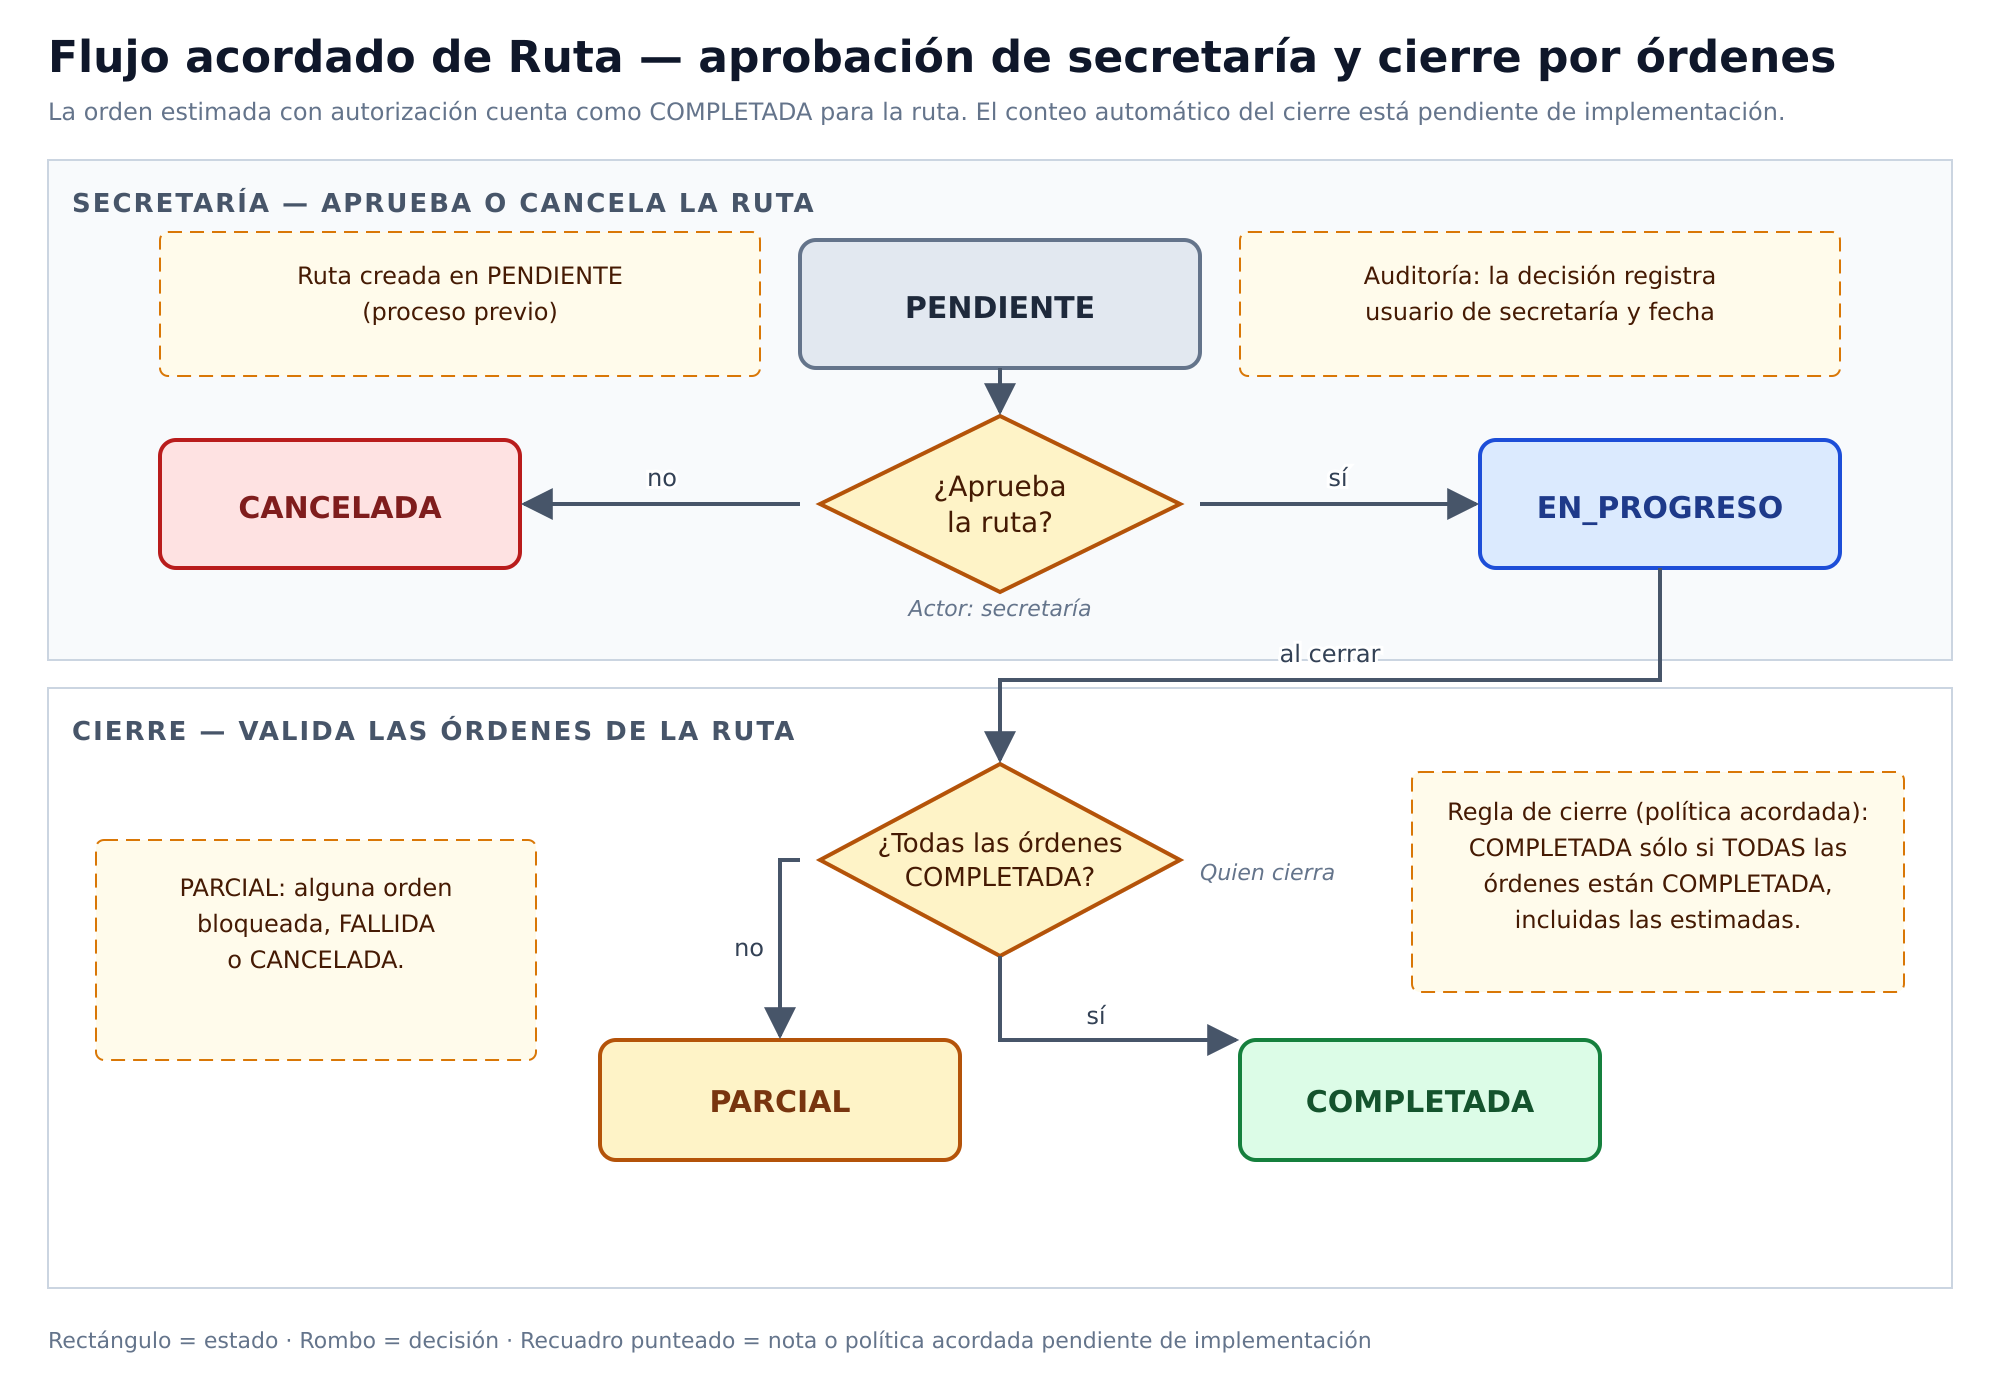
\includegraphics[width=0.95\textwidth]{images/04-ruta-flujo.png}}{\fbox{\parbox{0.88\textwidth}{\centering Flujo acordado de la ruta: PENDIENTE $\rightarrow$ EN\_PROGRESO (aprueba secretaría) o CANCELADA; cierre COMPLETADA/PARCIAL según las órdenes.\\[3pt]Agregar \texttt{images/04-ruta-flujo.png} para reemplazar este fallback.}}}
\caption{Flujo acordado de la ruta. Fuente editable: {\ttfamily diagrams/ruta-estados.drawio}.}
\end{figure}

Resumen textual del flujo:
\begin{itemize}
\item La ruta nace en \texttt{PENDIENTE}.
\item Secretaría decide con auditoría (usuario y fecha): si no la aprueba, la ruta pasa a \texttt{CANCELADA}; si la aprueba, pasa a \texttt{EN\_PROGRESO}.
\item Al cerrar una ruta en \texttt{EN\_PROGRESO} se validan sus órdenes (\textbf{conteo pendiente de implementación}): si TODAS están \texttt{COMPLETADA} —incluidas las completadas por estimación autorizada—, la ruta pasa a \texttt{COMPLETADA}; si alguna sigue bloqueada, o está \texttt{FALLIDA} o \texttt{CANCELADA}, la ruta pasa a \texttt{PARCIAL}.
\end{itemize}

Alcance en código: \texttt{UpdateRouteStateUseCase} confirma las transiciones del operador. \texttt{COMPLETADA} y \texttt{CANCELADA} son terminales en ese caso de uso.

\subsubsection{Estado de la orden}
Alcance: transiciones \textbf{acordadas} (política); los estados del enum y las escrituras están confirmados, pero \texttt{UpdateOrdenEstadoUseCase} no define una tabla de transiciones en código.

\begin{itemize}
\item \texttt{PENDIENTE} $\rightarrow$ \texttt{EN\_PROGRESO}: el operador inicia el trabajo.
\item \texttt{EN\_PROGRESO} $\rightarrow$ \texttt{COMPLETADA}: sin novedad activa, con la novedad resuelta, o con estimación autorizada por secretaría.
\item \texttt{EN\_PROGRESO} $\rightarrow$ \texttt{FALLIDA}: el caso es irrecuperable.
\item \texttt{EN\_PROGRESO} $\rightarrow$ \texttt{CANCELADA}: se cancela el trabajo.
\item Con novedad activa sin resolver, la orden permanece en \texttt{EN\_PROGRESO} con \texttt{tieneNovedadActiva=true} (ver flujo acordado).
\end{itemize}

\subsubsection{Estado de las novedades de órdenes de trabajo}

Sí existe una máquina de estados independiente para \texttt{NovedadOrdenTrabajo}. El modelo Prisma confirma \texttt{OPEN}, \texttt{IN	extunderscore PROGRESS}, \texttt{RESOLVED} y \texttt{CANCELLED}. La novedad se relaciona con una orden y opcionalmente con una lectura y el usuario que la resolvió.

Alcance: \textbf{Confirmado} para los estados, el valor inicial \texttt{OPEN} y los datos de resolución. No se encontró un controlador o caso de uso dedicado que confirme las transiciones HTTP; las flechas de atención y resolución son un flujo esperado.

La máquina, en texto:
\begin{itemize}
\item \texttt{OPEN} (valor inicial al crear la novedad) $\rightarrow$ \texttt{IN\_PROGRESS}: inicia la atención (flujo esperado).
\item \texttt{IN\_PROGRESS} $\rightarrow$ \texttt{RESOLVED}: registra la resolución con usuario y fecha (flujo esperado).
\item \texttt{OPEN} o \texttt{IN\_PROGRESS} $\rightarrow$ \texttt{CANCELLED}: se cancela (flujo esperado, sin reactivación confirmada).
\end{itemize}

La novedad de medidor dañado puede seguir en \texttt{OPEN} después de una estimación autorizada, para gestionar el reemplazo futuro del medidor.

\begin{center}
\small
\begin{longtable}{|p{0.31\textwidth}|p{0.63\textwidth}|}
\hline
\textbf{Elemento} & \textbf{Valores o datos confirmados} \\
\hline
\endfirsthead
\hline
\textbf{Elemento} & \textbf{Valores o datos confirmados} \\
\hline
\endhead
Estado & \texttt{OPEN}, \texttt{IN\textunderscore PROGRESS}, \texttt{RESOLVED}, \texttt{CANCELLED}. \\
\hline
Tipo de anomalía & \texttt{FUGA}, \texttt{MEDIDOR\textunderscore DAÑADO}, \texttt{LECTURA\textunderscore ERRONEA}, \texttt{OTRO}. \\
\hline
Resolución económica & \texttt{COBRO\textunderscore REAL}, \texttt{PROMEDIO\textunderscore HISTORICO}, \texttt{EXONERACION\textunderscore PARCIAL}, \texttt{EXONERACION\textunderscore TOTAL}, \texttt{AJUSTE\textunderscore LECTURA}. \\
\hline
Datos de resolución & \texttt{resolucionTipo}, \texttt{consumoAjustado}, \texttt{observacionResolucion}, \texttt{resueltoPorUsuarioId}, \texttt{resueltoEn}. \\
\hline
\end{longtable}
\end{center}

\texttt{resultadoObservacion} y \texttt{estado=FALLIDA} de \texttt{OrdenesTrabajo} no sustituyen a \texttt{NovedadOrdenTrabajo}: representan el resultado de la orden, mientras que la novedad conserva la anomalía y su resolución.


\subsection{Casos de uso}


\subsubsection{Caso: Consultar períodos}


\textbf{Descripción:} lista períodos disponibles para filtros y asignación.  

\textbf{HTTP y ruta:} \texttt{\detokenize{GET /api/v1/routes/periods}}.  

\textbf{Permiso:} \texttt{\detokenize{routes:read}}.  

\textbf{Cadena:} \texttt{\detokenize{RoutesController.getPeriods()}} → \texttt{\detokenize{RoutesService.getPeriodos()}} → repositorio.  

\textbf{Errores relevantes:} \texttt{\detokenize{401}}; \texttt{\detokenize{403}}.  

\textbf{Efectos:} ninguno.  

\textbf{Prisma:} \texttt{\detokenize{Periodos}}.  

\textbf{Entrada:} sin body ni parámetros.  

\textbf{Salida:}


\begin{lstlisting}
[{"periodoId":12,"nombre":"2026-08","estado":"ACTIVO"}]
\end{lstlisting}


\subsubsection{Caso: Consultar lecturas elegibles}


\textbf{Descripción:} devuelve lecturas disponibles para asignarlas a una ruta.  

\textbf{HTTP y ruta:} \texttt{\detokenize{GET /api/v1/routes/eligible-readings}}.  

\textbf{Permiso:} \texttt{\detokenize{routes:read}}.  

\textbf{Cadena:} \texttt{\detokenize{RoutesController.getEligibleReadings()}} → \texttt{\detokenize{RoutesService.getEligibleReadings()}} → \texttt{\detokenize{GetEligibleReadingsUseCase.execute()}}.  

\textbf{Errores relevantes:} \texttt{\detokenize{400}}; \texttt{\detokenize{401}}; \texttt{\detokenize{403}}.  

\textbf{Efectos:} ninguno.  

\textbf{Prisma:} \texttt{\detokenize{Lecturas}}, \texttt{\detokenize{Contratos}}, \texttt{\detokenize{Medidores}}, \texttt{\detokenize{Periodos}}, \texttt{\detokenize{OrdenTrabajo}}.  

\textbf{Entrada:} sin body; query \texttt{\detokenize{page}}, \texttt{\detokenize{limit}} y filtros de \texttt{\detokenize{FilterReadingsDto}}.  

\textbf{Salida:}


\begin{lstlisting}
{"data":[{"lecturaId":"101","estado":"PENDIENTE"}],"meta":{"page":1,"limit":10,"total":1,"totalPages":1},"kpis":{}}
\end{lstlisting}


\subsubsection{Caso: Consultar lecturas de ruta}


\textbf{Descripción:} lista lecturas ya vinculadas a una ruta.  

\textbf{HTTP y ruta:} \texttt{\detokenize{GET /api/v1/routes/:rutaId/readings}}.  

\textbf{Permiso:} \texttt{\detokenize{routes:read}}.  

\textbf{Cadena:} \texttt{\detokenize{RoutesController.getReadingsByRuta()}} → \texttt{\detokenize{RoutesService.getReadingsByRuta()}} → \texttt{\detokenize{GetReadingsByRutaUseCase.execute()}}.  

\textbf{Errores relevantes:} \texttt{\detokenize{400}}; \texttt{\detokenize{401}}; \texttt{\detokenize{403}}; \texttt{\detokenize{404}}.  

\textbf{Efectos:} ninguno.  

\textbf{Prisma:} \texttt{\detokenize{Rutas}}, \texttt{\detokenize{OrdenTrabajo}}, \texttt{\detokenize{Lecturas}}.  

\textbf{Entrada:} sin body; path \texttt{\detokenize{{ "rutaId": "42" }}}; query \texttt{\detokenize{page}}, \texttt{\detokenize{limit}}.  

\textbf{Salida:}


\begin{lstlisting}
{"data":[{"lecturaId":"101","estado":"PENDIENTE"}],"meta":{"page":1,"limit":10,"total":1,"totalPages":1},"kpis":{}}
\end{lstlisting}


\subsubsection{Caso: Crear ruta}


\textbf{Descripción:} crea una ruta de trabajo con su período y tipo.  

\textbf{HTTP y ruta:} \texttt{\detokenize{POST /api/v1/routes}}.  

\textbf{Permiso:} \texttt{\detokenize{routes:create}}.  

\textbf{Cadena:} \texttt{\detokenize{RoutesController.create()}} → \texttt{\detokenize{RoutesService.create()}} → \texttt{\detokenize{CreateRouteUseCase.execute()}} → repositorio.  

\textbf{Errores relevantes:} \texttt{\detokenize{400}}; \texttt{\detokenize{401}}; \texttt{\detokenize{403}}; \texttt{\detokenize{404}} período/guías.  

\textbf{Efectos:} alta en \texttt{\detokenize{Rutas}} y asociaciones que determine el caso.  

\textbf{Prisma:} \texttt{\detokenize{Rutas}}, \texttt{\detokenize{OrdenTrabajo}}, \texttt{\detokenize{Contratos}}, \texttt{\detokenize{Periodos}}.  

\textbf{Entrada:} body \texttt{\detokenize{{ "nombre": "Lecturas agosto", "tipoRuta": "LECTURA", "periodoId": 12 }}}.  

\textbf{Salida:}


\begin{lstlisting}
{"rutaId":"42","nombre":"Lecturas agosto","estado":"PENDIENTE","ordenesTrabajo":[]}
\end{lstlisting}


\subsubsection{Caso: Listar rutas}


\textbf{Descripción:} devuelve rutas con paginación y filtros.  

\textbf{HTTP y ruta:} \texttt{\detokenize{GET /api/v1/routes}}.  

\textbf{Permiso:} \texttt{\detokenize{routes:read}}.  

\textbf{Cadena:} \texttt{\detokenize{RoutesController.findAll()}} → \texttt{\detokenize{RoutesService.findAll()}} → repositorio.  

\textbf{Errores relevantes:} \texttt{\detokenize{400}}; \texttt{\detokenize{401}}; \texttt{\detokenize{403}}.  

\textbf{Efectos:} ninguno.  

\textbf{Prisma:} \texttt{\detokenize{Rutas}} y relaciones.  

\textbf{Entrada:} sin body; query \texttt{\detokenize{page}}, \texttt{\detokenize{limit}}, \texttt{\detokenize{estado}}, \texttt{\detokenize{operarioId}}, \texttt{\detokenize{comunidadId}}, \texttt{\detokenize{periodoId}}, \texttt{\detokenize{tipoRuta}}.  

\textbf{Salida:}


\begin{lstlisting}
{"data":[{"rutaId":"42","estado":"PENDIENTE"}],"meta":{"page":1,"limit":10,"total":1,"totalPages":1}}
\end{lstlisting}


\subsubsection{Caso: Obtener ruta}


\textbf{Descripción:} consulta una ruta por ID.  

\textbf{HTTP y ruta:} \texttt{\detokenize{GET /api/v1/routes/:id}}.  

\textbf{Permiso:} \texttt{\detokenize{routes:read}}.  

\textbf{Cadena:} \texttt{\detokenize{RoutesController.findOne()}} → \texttt{\detokenize{RoutesService.findOne()}} → repositorio.  

\textbf{Errores relevantes:} \texttt{\detokenize{400}}; \texttt{\detokenize{401}}; \texttt{\detokenize{403}}; \texttt{\detokenize{404}}.  

\textbf{Efectos:} ninguno.  

\textbf{Prisma:} \texttt{\detokenize{Rutas}}, \texttt{\detokenize{OrdenTrabajo}}, \texttt{\detokenize{Contratos}}, \texttt{\detokenize{Periodos}}.  

\textbf{Entrada:} sin body; path \texttt{\detokenize{{ "id": "42" }}}.  

\textbf{Salida:}


\begin{lstlisting}
{"rutaId":"42","estado":"PENDIENTE","ordenesTrabajo":[]}
\end{lstlisting}


\subsubsection{Caso: Actualizar ruta}


\textbf{Descripción:} modifica los datos de una ruta existente.  

\textbf{HTTP y ruta:} \texttt{\detokenize{PATCH /api/v1/routes/:id}}.  

\textbf{Permiso:} \texttt{\detokenize{routes:update}}.  

\textbf{Cadena:} \texttt{\detokenize{RoutesController.update()}} → \texttt{\detokenize{RoutesService.update()}} → \texttt{\detokenize{UpdateRouteUseCase.execute()}} → repositorio.  

\textbf{Errores relevantes:} \texttt{\detokenize{400}}; \texttt{\detokenize{401}}; \texttt{\detokenize{403}}; \texttt{\detokenize{404}}.  

\textbf{Efectos:} actualización de \texttt{\detokenize{Rutas}}; DTO puro.  

\textbf{Prisma:} \texttt{\detokenize{Rutas}}.  

\textbf{Entrada:} path \texttt{\detokenize{{ "id": "42" }}}; body \texttt{\detokenize{{ "nombre": "Ruta actualizada" }}}.  

\textbf{Salida:} \texttt{\detokenize{{ "rutaId": "42", "nombre": "Ruta actualizada", "estado": "PENDIENTE" }}}.


\subsubsection{Caso: Reasignar ruta}


\textbf{Descripción:} asigna o desasigna la ruta a un operario.  

\textbf{HTTP y ruta:} \texttt{\detokenize{PATCH /api/v1/routes/:id/reassign}}.  

\textbf{Permiso:} \texttt{\detokenize{routes:update}}.  

\textbf{Cadena:} \texttt{\detokenize{RoutesController.reassign()}} → \texttt{\detokenize{ReassignRouteUseCase.execute()}} → repositorio.  

\textbf{Errores relevantes:} \texttt{\detokenize{400}}; \texttt{\detokenize{401}}; \texttt{\detokenize{403}}; \texttt{\detokenize{404}}; ruta ya asignada.  

\textbf{Efectos:} cambia \texttt{\detokenize{Rutas.operarioId}}.  

\textbf{Prisma:} \texttt{\detokenize{Rutas}}, \texttt{\detokenize{Usuarios/Operarios}}.  

\textbf{Entrada:} path \texttt{\detokenize{{ "id": "42" }}}; body \texttt{\detokenize{{ "operarioId": "7" }}} o \texttt{\detokenize{null}}.  

\textbf{Salida:} \texttt{\detokenize{{ "rutaId": "42", "operarioId": 7, "estado": "PENDIENTE" }}}.


\subsubsection{Caso: Eliminar ruta}


\textbf{Descripción:} elimina lógicamente la ruta.  

\textbf{HTTP y ruta:} \texttt{\detokenize{DELETE /api/v1/routes/:id}}.  

\textbf{Permiso:} \texttt{\detokenize{routes:delete}}.  

\textbf{Cadena:} \texttt{\detokenize{RoutesController.delete()}} → \texttt{\detokenize{RoutesService.delete()}} → \texttt{\detokenize{DeleteRouteUseCase.execute()}} → repositorio.  

\textbf{Errores relevantes:} \texttt{\detokenize{400}}; \texttt{\detokenize{401}}; \texttt{\detokenize{403}}; \texttt{\detokenize{404}}.  

\textbf{Efectos:} soft delete y desasignación según el caso.  

\textbf{Prisma:} \texttt{\detokenize{Rutas}}, \texttt{\detokenize{OrdenTrabajo}}, \texttt{\detokenize{Lecturas}}.  

\textbf{Entrada:} sin body; path \texttt{\detokenize{{ "id": "42" }}}.  

\textbf{Salida:} \texttt{\detokenize{{ "rutaId": "42", "estado": "CANCELADA" }}}.


\subsubsection{Caso: Exportar hoja de campo}


\textbf{Descripción:} genera la hoja oficial de órdenes y lecturas.  

\textbf{HTTP y ruta:} \texttt{\detokenize{GET /api/v1/routes/:id/pdf}}.  

\textbf{Permiso:} \texttt{\detokenize{routes:read}}.  

\textbf{Cadena:} \texttt{\detokenize{RoutesController.exportPdf()}} → \texttt{\detokenize{RoutesService.exportPdf()}} → \texttt{\detokenize{ExportFieldSheetPdfUseCase}}/generador.  

\textbf{Errores relevantes:} \texttt{\detokenize{400}}; \texttt{\detokenize{401}}; \texttt{\detokenize{403}}; \texttt{\detokenize{404}}.  

\textbf{Efectos:} lectura y generación puras.  

\textbf{Prisma:} \texttt{\detokenize{Rutas}}, \texttt{\detokenize{OrdenTrabajo}}, \texttt{\detokenize{Lecturas}}.  

\textbf{Entrada:} sin body; path \texttt{\detokenize{{ "id": "42" }}}.  

\textbf{Salida:} no es JSON: \texttt{\detokenize{application/pdf}}, \texttt{\detokenize{Content-Disposition: inline}}, \texttt{\detokenize{Content-Length}} y bytes PDF.


\subsubsection{Caso: Consultar órdenes de una ruta}


\textbf{Descripción:} lista órdenes asociadas, filtradas y paginadas.  

\textbf{HTTP y ruta:} \texttt{\detokenize{GET /api/v1/routes/:id/work-orders}}.  

\textbf{Permiso:} \texttt{\detokenize{routes:read}}.  

\textbf{Cadena:} \texttt{\detokenize{RoutesController.findOrdenesByRuta()}} → \texttt{\detokenize{OrdenesTrabajoService.findByRuta()}} → \texttt{\detokenize{FindOrdenesByRutaUseCase.execute()}}.  

\textbf{Errores relevantes:} \texttt{\detokenize{400}}; \texttt{\detokenize{401}}; \texttt{\detokenize{403}}; \texttt{\detokenize{404}}.  

\textbf{Efectos:} ninguno.  

\textbf{Prisma:} \texttt{\detokenize{OrdenTrabajo}}, \texttt{\detokenize{Rutas}}, \texttt{\detokenize{Lecturas}}.  

\textbf{Entrada:} sin body; path \texttt{\detokenize{{ "id": "42" }}}; query \texttt{\detokenize{estado}}, \texttt{\detokenize{page}}, \texttt{\detokenize{limit}}.  

\textbf{Salida:} \texttt{\detokenize{{ "data": [{ "ordenTrabajoId": "9", "estado": "PENDIENTE" }], "meta": {}, "kpis": {} }}}.


\subsubsection{Caso: Actualizar estado de orden}


\textbf{Descripción:} cambia estado, observación y fecha de finalización de una orden.  

\textbf{HTTP y ruta:} \texttt{\detokenize{PATCH /api/v1/work-orders/:id/state}}.  

\textbf{Permiso:} \texttt{\detokenize{routes:update}}.  

\textbf{Cadena:} \texttt{\detokenize{OrdenesTrabajoController.updateEstado()}} → \texttt{\detokenize{OrdenesTrabajoService.updateEstado()}} → \texttt{\detokenize{UpdateOrdenEstadoUseCase.execute()}} → repositorio.  

\textbf{Errores relevantes:} \texttt{\detokenize{400}}; \texttt{\detokenize{401}}; \texttt{\detokenize{403}}; \texttt{\detokenize{404}}; \texttt{\detokenize{409}}.  

\textbf{Efectos:} persiste estado; completa o limpia \texttt{\detokenize{completadoEn}}.  

\textbf{Prisma:} \texttt{\detokenize{OrdenTrabajo}}, \texttt{\detokenize{EjecucionOrdenTrabajo}}.  

\textbf{Entrada:} path \texttt{\detokenize{{ "id": "9" }}}; body \texttt{\detokenize{{ "estado": "COMPLETADA", "resultadoObservacion": "Trabajo realizado" }}}.  

\textbf{Salida:} \texttt{\detokenize{{ "ordenTrabajoId": "9", "estado": "COMPLETADA" }}}.


\subsubsection{Caso: Vincular lectura a orden}


\textbf{Descripción:} asocia una lectura y completa la orden.  

\textbf{HTTP y ruta:} \texttt{\detokenize{PATCH /api/v1/work-orders/:id/reading}}.  

\textbf{Permiso:} \texttt{\detokenize{routes:update}}.  

\textbf{Cadena:} \texttt{\detokenize{OrdenesTrabajoController.linkLectura()}} → \texttt{\detokenize{OrdenesTrabajoService.linkLectura()}} → \texttt{\detokenize{LinkLecturaUseCase.execute()}} → repositorio.  

\textbf{Errores relevantes:} \texttt{\detokenize{400}}; \texttt{\detokenize{401}}; \texttt{\detokenize{403}}; \texttt{\detokenize{404}}; \texttt{\detokenize{409}}.  

\textbf{Efectos:} persiste vínculo y \texttt{\detokenize{completadoEn}}.  

\textbf{Prisma:} \texttt{\detokenize{OrdenTrabajo}}, \texttt{\detokenize{Lecturas}}, \texttt{\detokenize{Rutas}}.  

\textbf{Entrada:} path \texttt{\detokenize{{ "id": "9" }}}; body \texttt{\detokenize{{ "lecturaId": "101" }}}.  

\textbf{Salida:} \texttt{\detokenize{{ "ordenTrabajoId": "9", "lecturaId": "101", "estado": "COMPLETADA" }}}.


\subsubsection{Caso: Actualizar operación del operador}


\textbf{Descripción:} registra ejecución y evidencia opcional de una orden.  

\textbf{HTTP y ruta:} \texttt{\detokenize{PATCH /api/v1/operator/work-orders/:id}}.  

\textbf{Permiso:} \texttt{\detokenize{routes:update}}.  

\textbf{Cadena:} \texttt{\detokenize{OperatorController.updateOperatorWorkOrder()}} → \texttt{\detokenize{UpdateOperatorWorkOrderUseCase.execute()}} → repositorio/RustFS.  

\textbf{Errores relevantes:} \texttt{\detokenize{400}}; \texttt{\detokenize{401}}; \texttt{\detokenize{403}}; \texttt{\detokenize{404}}; \texttt{\detokenize{409}}.  

\textbf{Efectos:} persiste ejecución y \texttt{\detokenize{evidenciaFotoUrl}}; la subida y rollback de archivo son efectos reales.  

\textbf{Prisma:} \texttt{\detokenize{OrdenTrabajo}}, \texttt{\detokenize{EjecucionOrdenTrabajo}}, \texttt{\detokenize{NovedadOrdenTrabajo}}.  

\textbf{Entrada:} path \texttt{\detokenize{{ "id": "9" }}}; multipart: campos DTO y archivo opcional \texttt{\detokenize{foto}}; sin body JSON.  

\textbf{Salida:} JSON \texttt{\detokenize{OrderWorkResponseDto}}, por ejemplo \texttt{\detokenize{{ "ordenTrabajoId": "9", "estado": "COMPLETADA", "evidenciaFotoUrl": "ordenes/9/foto.jpg" }}}.


\subsubsection{Caso: Listar rutas del operador}


\textbf{Descripción:} lista las rutas del período activo asignadas al operador autenticado.  

\textbf{HTTP y ruta:} \texttt{\detokenize{GET /api/v1/operator/routes}}.  

\textbf{Permiso:} \texttt{\detokenize{routes:read}}.  

\textbf{Cadena:} \texttt{\detokenize{OperatorController.getOperatorRoutes()}} → \texttt{\detokenize{GetOperatorRoutesUseCase.execute()}} → repositorio.  

\textbf{Errores relevantes:} \texttt{\detokenize{400}}; \texttt{\detokenize{401}}; \texttt{\detokenize{403}}; \texttt{\detokenize{404}} sin período activo.  

\textbf{Efectos:} ninguno; consulta y DTO puros.  

\textbf{Prisma:} \texttt{\detokenize{Rutas}}, \texttt{\detokenize{OrdenTrabajo}}, \texttt{\detokenize{Periodos}}.  

\textbf{Entrada:} sin body; query opcional \texttt{\detokenize{tipoRuta}}; operador desde JWT.  

\textbf{Salida:} lista JSON de \texttt{\detokenize{OperatorRouteResponseDto}}.


\subsubsection{Caso: Actualizar estado de ruta del operador}


\textbf{Descripción:} cambia el estado de una ruta que pertenece al operador autenticado.  

\textbf{HTTP y ruta:} \texttt{\detokenize{PATCH /api/v1/operator/routes/:id/state}}.  

\textbf{Permiso:} \texttt{\detokenize{routes:update}}.  

\textbf{Cadena:} \texttt{\detokenize{OperatorController.updateRouteState()}} → \texttt{\detokenize{UpdateRouteStateUseCase.execute()}} → repositorio.  

\textbf{Errores relevantes:} \texttt{\detokenize{400}}; \texttt{\detokenize{401}}; \texttt{\detokenize{403}} ruta ajena; \texttt{\detokenize{404}}; \texttt{\detokenize{409}} transición inválida.  

\textbf{Efectos:} actualiza \texttt{\detokenize{Rutas}} y las marcas temporales derivadas del estado.  

\textbf{Prisma:} \texttt{\detokenize{Rutas}}, \texttt{\detokenize{OrdenTrabajo}}, \texttt{\detokenize{Periodos}}.  

\textbf{Entrada:} path \texttt{\detokenize{{ "id": "42" }}}; body \texttt{\detokenize{{ "estado": "EN_PROGRESO" }}}.  

\textbf{Salida:} \texttt{\detokenize{{ "rutaId": "42", "estado": "EN_PROGRESO" }}}.


\subsection{Pendientes funcionales}

Bloqueos confirmados como pendientes en el código revisado. Cuando se cierre cada uno, sacar de acá y mover a la sección correspondiente.

\begin{itemize}
\item \textbf{Bloqueo por novedad activa al transicionar la orden a \texttt{COMPLETADA}.} El helper \texttt{applyContractLifecycleTransition} solo valida estado origen del contrato, no valida \texttt{tieneNovedadActiva}. Falta decidir el criterio bloqueante (\texttt{afectaOrden}, tipo de novedad o resolución) e implementar la validación en \texttt{UpdateOrdenEstadoUseCase} o en el repositorio de órdenes.
\item \textbf{Autorización exclusiva del rol \texttt{Secretaría} para la estimación con los últimos 3 meses.} Mismo punto pendiente en \texttt{05-lecturas.md}. Requiere endpoint nuevo o permiso específico (\texttt{estimates:approve} o equivalente). La política está acordada pero no está aplicada en código.
\item \textbf{Conteo automático de órdenes para el cierre de la ruta} (\texttt{COMPLETADA} vs \texttt{PARCIAL}). Si TODAS las órdenes están \texttt{COMPLETADA} (incluidas completadas por estimación), la ruta pasa a \texttt{COMPLETADA}; si alguna está \texttt{FALLIDA} o \texttt{CANCELADA}, pasa a \texttt{PARCIAL}. Hoy \texttt{UpdateRouteUseCase} no implementa esa lógica; el estado final lo asigna manualmente quien cierre la ruta.
\item \textbf{Endpoints HTTP para gestión manual de \texttt{NovedadOrdenTrabajo}.} Hoy la entidad solo tiene repositorio; la creación y actualización de novedades ocurre internamente desde otros flujos (captura de lecturas, reporte de defectos). Si el operador debe poder crear/actualizar/resolver novedades desde la UI, falta el controller + use cases correspondientes.
\item \textbf{Auditoría de la decisión de secretaría al aprobar una ruta para \texttt{EN\_PROGRESO}} (usuario y fecha). El documento lo menciona en la sección de flujo acordado de la ruta pero no indica tabla ni columnas donde se persiste esa decisión.
\item \textbf{Tipo de novedad \texttt{INSPECCION} sin efecto sobre ciclo de vida del contrato.} El helper \texttt{applyContractLifecycleTransition} solo reconoce los tipos \texttt{INSTALACION} y \texttt{RECONEXION}. Si una orden de inspección tiene contrato asociado, el efecto sobre el estado del contrato queda indefinido.
\end{itemize}

\subsection{No documentado o pendiente de confirmar}


\begin{itemize}
\item Lista exhaustiva de transiciones de operador.
\item Endpoints legacy basados en \texttt{\detokenize{EstadoAsignacion}}.
\end{itemize}
